\documentclass[11pt]{article}
\usepackage[top=1.00in, bottom=1.0in, left=1in, right=1in]{geometry}
\renewcommand{\baselinestretch}{1.1}
\usepackage{graphicx}
\usepackage{natbib}
\usepackage{amsmath}
\usepackage{gensymb}
\usepackage{xcolor}
\usepackage{xr-hyper}
\externaldocument{bayesianflowsysupp}

\def\labelitemi{--}

\usepackage{fancyhdr}
\pagestyle{fancy}
\fancyhead[LO]{}
\fancyhead[RO]{}

\begin{document}
\bibliographystyle{/Users/Lizzie/Documents/EndnoteRelated/Bibtex/styles/amnat}
\renewcommand{\refname}{\CHead{}}

%%%%%%%
%% Built 8 March 2026 for FINAL submission to PhilTrans A
%% Removed all comments, line numbers, added bbl
%%%%%%%

\title{A four-step simulation-based workflow for \\ecological analysis and science}
\author{EM Wolkovich$^{1*}$, T Jonathan Davies$^{1,2}$, William D Pearse$^{3,4}$ \& Michael Betancourt$^{5}$}
\maketitle

\noindent $^{1}$ Forest and Conservation Sciences, University of British Columbia, Vancouver, BC V6T 1Z4, Canada\\
$^{2}$ Botany, University of British Columbia, Vancouver, BC V6T 1Z4, Canada\\
$^{3}$ Department of Life Sciences, Imperial College London, Ascot SL5 7PY, United Kingdom \\
$^{4}$ Alan Turing Institute, British Library, 96 Euston Road, London NW1 2DB, United Kingdom \\
$^{5}$ Symplectomorphic, LLC, New York, NY 10026, USA \\
$^{*}$ \url{mailto: e.wolkovich@ubc.ca}
 
\vspace{3ex}
\noindent \emph{Keywords:} big data; scientific workflow; data simulation; prediction; null hypothesis testing, machine learning
\vspace{3ex}


\newpage
\abstract{Ecology is a discipline that has faced increasing challenges as the disconnect between its scientific and statistical methods has become more obvious. Growing demands for useful forecasts in an era of intensifying global change requires models that can capture the variability and underlying uncertainty of ecological systems and related data. Yet many ecologists are not trained in current methods to build the flexible robust models needed to address this challenge. Thus, there is often a reliance on a limited set of pre-defined models combined with null hypothesis testing or a temptation to adopt new approaches without fully understanding their limitations. The result is poor models that lead to incorrect predictions, alongside concerns of a looming replication crisis.
Here we show how new advances in workflows can lead to better models and enhance training in ecology. 
Building on the increasingly computational toolkit of many ecologists, this approach leverages simulation to integrate model building and testing of empirical data more fully with ecological theory. We argue this approach can fit models that are more robust and better-suited to providing new ecological insights and improved predictions, and may provide a blueprint for other fields similarly challenged by complex systems, growing datasets and limited training in how to best approach them. }


\vspace{3ex}
\noindent\emph{Examples \& Data:} We provide an example of the full workflow with complete code available at \url{https://github.com/lizzieinvancouver/bayesianflowsexample}. The data used for the example is provided and full metadata on it is available via the Knowledge Network for Biocomplexity: \verb|doi:10.5063/F12J69B2|. All other examples use simulated data.



\setlength{\parindent}{0pt}
\setlength{\parskip}{7pt}

\newpage

\section*{Introduction}
Ecology is a discipline that has followed a similar trajectory to other biological and social science fields in its growing aims, study design and data collection. Historically, ecological research commonly reported results from experiments or observations of one site using frequentist test statistics associated with null hypothesis testing. Mechanistic models were typically the domain of theorists, who studied ordinary differential equations (ODE, for example of Lotka Volterra predator-prey dynamics or the relationship between stability and complexity) and rarely compared their models explicitly to empirical data \citep[see][]{caswell1988}. But in recent decades growing demands have pushed ecological science to work across systems, contribute to policy and provide models to forecast the outcomes of growing anthropogenic pressures \citep{hak2016sustainable,lindenmayer2010science}. These new scales and aims have led some ecologists to try to adapt what they were trained in (e.g., null hypothesis testing using $F$ and $t$ tests) to increasingly larger scales, more complex datasets, and to fads in specific approaches  \citep{grace2025causal}. 

Yet many commonly used statistical approaches do not align with these new demands. Beyond the reality that most traditional methods are fragile when used beyond the cleaner, simpler experiments these methods assume (e.g. spatial, temporal and phylogenetic correlations often violate independence assumptions), they will usually fail to produce robust, reproducible results. For example, an overly zealous focus on $p$-values has led to a replication crises in several fields, where results derived from studies with small sample sizes seem most likely the outcome of noisy data combined with a search for statistical significance through many models \citep[effectively a garden of forking paths,][]{halsey2015,loken2017}. Some model selection approaches, including new machine learning methods, try to avoid this by comparing across models, but may not generalize to provide useful forecasts. This is especially true when forecasts have to adapt to changes in the underlying biology  \citep{boettiger2022forecast}. This leaves ecology in a predicament shared across other fields---concerns of a looming replication crisis \citep{filazzola2021replication,fraser2020role} and overly confident forecasts with the potential to erode public trust in science when found not to be accurate \citep{leroux2019prevalence,boettiger2022forecast}. 

Many researchers recognize these issues and have turned to methods better designed for forecasting from complex systems and messy data. Machine learning methods, which benefit from large datasets---often with many predictors---fitted to test and training datasets \citep{breiman2001statistical}, have revolutionized image classification in ecology and remote sensing, but are increasingly used to forecast ecological processes \citep[e.g.,][]{zwart2023near}. These methods often build complex, opaque (`black-box') models \citep{CoxTwoCultures,EfronTwoCultures,shmueli2010explain}, thus providing opaque inference into ecological processes. Bayesian inference encourages the fitting of bespoke mechanistic models with interpretable parameters and can thus handle many of the complexities of ecological data \citep{hobbs2006alternatives}. Long used in select applications in ecology \citep{muthuku2008,zheng2007,trijoulet2018,strinella2020potential}, Bayesian inference has recently increased in use \citep{anderson2021trends,pichler2023machine}, alongside new algorithms \citep[e.g. Hamiltonian Monte Carlo,][]{nuts2014,betan2019} that have made fitting and implementing models faster, more robust and---in many ways---easier \citep{Carpenter:2017stan}

Regardless of the approach, fitting larger and more complex models has not dramatically improved forecasts, nor made research more reproducible. Instead, these new approaches have highlighted a fundamental training disconnect that applies from simple to complex models: treating scientific and statistical methods as separate.

Merging scientific and statistical training is possible by approaching analyses through specific workflows \citep{betanworkflow,grinsztajn2021,vandeschoot2021}, which themselves are built on a process of how to do not just statistics, but how to do science \citep{box1976science}. While these approaches are slowly gaining traction in other fields \citep[e.g.,][]{esfahani2021bayesian,schad2021,bouman2024bayesian}, they are not widely used in ecology and related fields today. Such approaches move away from a focus on null hypothesis testing, towards estimating effect sizes, using models calibrated (see Table \ref{tab:glossary}) and better understood through simulating data at multiple steps. We argue that potential benefits include not only a better understanding of models fit to empirical data, but also a better understanding of system dynamics by requiring explicit consideration of the generative processes underlying observations \citep{grace2025causal}. 

Here we outline a simplified---but powerful---workflow that builds on new insights from statistics  \citep{betanworkflow,gelman2020bayesian,vandeschoot2021} and the increasingly computational nature of ecology today. Our aim is to provide an approachable rubric for those new to fitting complex models or simply those interested in re-considering their current workflow (and is not intended to be a comprehensive overview; see `Next steps' in the Supplement). Because of this aim and to maximize interpretability, we illustrate our workflow using examples of simple models, and suggest additional resources as users build more complex models. Our examples include several statistical inference methods, though we focus on implementing the workflow through a Bayesian statistical framework (with an example shown in \textsf{R} and \textsf{Stan}), because this framework allows integrating bespoke model building more fully with ecological theory and understanding. We suggest that adopting this workflow approach can help fit models that are more robust and well-suited to provide new ecological insights---allowing us to refine where to put resources for better estimates, better models, and better forecasts.


\section*{A four-step workflow}

Our workflow outlines what we consider the major steps for building bespoke models (Fig. \ref{fig:workflow}). Several of these steps will be familiar to statistical ecologists, but are often overlooked, whereas other steps may appear particular to certain methods (e.g. prior predictive checks in Bayesian analyses), but are actually useful for anyone---using Bayesian models or not---to challenge their models of how the world works. We find that it is easiest to illustrate and describe this workflow using a Bayesian framework (see \emph{A brief review of statistical inference using Bayesian approaches} in the Supplement), but we argue this workflow can be adapted to other approaches (Fig. \ref{fig:twoexamples}).
Parts of this workflow could be expanded as workflows in themselves, given other aims (see Supplement: \emph{Which workflow?}). 

\subsection*{Step 1: Develop your model(s)} 

We start the workflow with what can feel like the biggest step---build a model (or potentially, models) based on your aims \citep{hilborn2013ecological}. By developing a model designed for your biological question, data and aims, your statistical workflow naturally becomes a scientific workflow. You will more clearly see the assumptions and mechanisms in your model, which is especially valuable given how often our intuition of how models `work' is wrong \citep{kokko2005useful}. You likely already have a model, though it may be only verbal or conceptual. For this workflow, however, you’ll need to convert such models into mathematical versions \citep{servedio2014not}. 

Though it can feel challenging at first, this step is best approached before you collect any data. A suite of resources for `generative' or `narratively generative' modeling can help \citep{statrethink,betangen}. 
As you start, ask lots of questions---and push yourself on your answers---about what you expect and what's reasonable biologically from your model. 
As you do this, you'll be generating your model---including its priors. Priors are important for Bayesian analysis, but the basic idea of them---coming up with a distribution of reasonable values for parameters in your model (see Table \ref{tab:glossary})---is useful to all analyses (for an example, see discussion of a heuristic model in the case study for Fig.  \ref{fig:twoexamples}b). Assigning priors generally forces you to think about your model with regard to your study system, and interrogate what's probable, possible or actually unreasonable---and can quickly disabuse users of prejudices regarding priors. For example, you may not think you have a prior on how sunlight affects plant growth, until you realize your `agnostic prior' actually allows plants to grow hundreds of meters per day. 

\subsection*{Step 2: Check your model on simulated data} 

Once you have your model and its priors jotted down, you need to formalise it in your preferred modeling language and check it. As with all code: just because it runs, does not mean it does what you think it does. The worst errors often still permit code to run. 

Test data (aka `simulated data', or  `fake data,' etc.), and the skills required to generate it, are central to this workflow. With `test data' you simulate data from your model in such a way that you can use the resulting data to test if your model code is correct (i.e., you fix values for your model parameters, then test how well your model recovers them, see the Supplement for several examples). This is more straightforward when your statistical model is the same as your generative model, but the basic idea can be adapted to other approaches (see Fig. \ref{fig:twoexamples}b). While there's no guarantee that inferences will always recover the parameter values you set, even when using the correct model, extreme disagreement is often an indicator that something is amiss in the implementation of the model. At the same time these simulation studies can help understand how often a model might lead to the correct inference (see Figs. \ref{fig:twoexamples} and S1). As you do this, you will also be calibrating your model---seeing how accurately and precisely it estimates parameters and under what conditions. 

This very basic model checking step is uncommon for many ecologists, but critical in our view. If you can simulate data from your model, then you can powerfully---and easily---answer questions related to statistical power (see Fig. \ref{fig:twoexamples}a and related Supplemental examples), what effect sizes are reasonable, and---most likely---have new insights into how your model suggests the world works, all before looking at any real data. Thus, this apparently simple programmatic task actually encapsulates a far deeper understanding of your model. `All models are wrong; some models are useful,' becomes much clearer when you have the power to generate data from your model under any parameter set and sample size you want.

You can learn only so much, however, from data simulated from a particular parameter set. Simulation studies across multiple parameter sets allow you to investigate how robust your inferential performance might be. Prior predictive checks \citep{betanprior,winter2023} use the Bayesian prior model to set the scope of such simulations, but the basic idea of prior predictive checks can be used in any analysis. For these, you draw values from your prior distribution and then explore how your model performs. Seeing how this influences your resulting model output 
reveals the extent to which your model can capture known variation in your data, and gives insight into whether your model is capable of distinguishing among competing hypotheses. If adopting a Bayesian approach, it can also serve as a check on the priors you're using (addressing one of the common concerns of those inexperienced with Bayesian models). 


 \subsection*{Step 3: Run your model on your empirical data} 
 
The next step is to run the model---you've now evaluated, test-run and have ready to go---on your exciting new empirical data. Check diagnostics so you know it's running well and adjust until it is. Which diagnostics to use depends on your exact fitting approach, with many approaches having a suite of metrics that are are well-discussed elsewhere \citep[for Bayesian methods, this includes a suite of convergence and efficiency metrics, see][]{betanworkflow,gelman2020bayesian,vandeschoot2021,gabryvis}. 
 
This is the step many ecologists skip straight to, ourselves included. It's easy to see the appeal: this is the inference step and where you might gain new ecological insights. Fitting new data to the model can feel like the moment when you'll learn something new. But, at least in our experience, this is not always the case. When we rush to this step, that first model we fit is often followed by another, and another---perhaps because one does not converge, or the results of another do not make immediate sense. And, with the excitement of getting a model to run, we can get distracted from what we are actually most interested in---the inference into our ecological system. 

Following this workflow can make this step much more satisfying. Here the benefits of the workflow may become especially apparent: using it with Bayesian inference you likely have estimates in useful units with uncertainty you can understand. You can use this information to draw new conclusions, design new experiments and more---but this is also a point to stop and check your model. 


\subsection*{Step 4: Check your model on data simulated from your empirical model output} 

Once you have your parameter estimates based on your model and new empirical data, it's time to remember that your model is wrong (as all models are) and ask how useful it is. You can do some of this through common model-fit diagnostics, such as $R^2$, which compares point predictions to the observed data. With a Bayesian posterior (see Table \ref{tab:glossary}), however, you have an added benefit in that you can compare an entire distribution of predictions to the observed data. 

This is where simulating from your model can be especially insightful. It will not only indicate when the model isn't adequately fitting the data but also can suggest what the problems might be. Using the parameter estimates from your fitted model to simulate new data \citep[][]{held2010,gelman200ppc,conn2018} lets you see how that new world compares to the observed data. This is most easily done in a Bayesian framework---called posterior retrodictive checks or posterior predictive checks (Fig. \ref{fig:retrodictivecheck})---where your posterior captures your uncertainty in a useful way, but can be done with estimates of your parameters and their uncertainty from other inferential frameworks. Exactly how to do this effectively, however, requires care for any particular framework. Tailoring these checks to the research question and model makes this step most likely to pick up model mis-specification and provide useful insight for improvement \citep[e.g.,][]{mimno2015posterior}.


Often here you may find large differences from your empirical data, and can start to generate hypotheses for why. For example, you may find patterns that suggest missing grouping factors (e.g. site or biome) through visual posterior retrodictive checks, or you may quickly realize your model predicts impossible numbers for your biological reality. You may begin to see inadequacies in your model, or even potentially your data.  This is one of the main benefits of the workflow: models don't fail silently, they fail with a wealth of context that helps to generate new models and experiments.


\subsection*{Feedbacks \& workflows}
A key feature of this workflow is that it can be iterated.  If you find that you want to tweak your model then you return to the beginning, adjust your model, and repeat the rest of the workflow (Fig. \ref{fig:workflow}). In this way, fitting multiple models is encouraged, but this is distinct from the quest for a minimum adequate model or one `best' fit. Feedbacks in this workflow are focused far more on what is biologically reasonable, and understanding the utility---and limits---of inference from your data for your model.  And there are big benefits to it. 


\section*{How this workflow changed our science} 
Before this workflow, not all of us commonly discussed the values that parameters in our model took---things like the slope and intercept (two common model parameters) were sometimes reported, but we did not know them as well as we knew whether the $p$-value for the slope was $<0.05$. This changes quickly when you need to build simulated data (Step 2). For example, when modeling phenological events (observations of biological events on numbered days within the calendar year: 1-366 days when including leap years) it is not uncommon to find seemingly-reasonable models generating predictions of events on non-existent calendar days beyond 366.

A closer inspection of our parameters also taught us a lot about identifiability and nonidentifiability, when all parameters in a model can---or cannot---be uniquely identified with infinite data, and a statistical kin: degeneracy (see Table \ref{tab:glossary}).  Degeneracy concerns the kinds of complex uncertainties that can arise from finite data sets \citep{gelmanhill}, and something we have often found in Steps 2-3 of our workflow.
Nonidentifiability and degeneracy can insert themselves in many ways in ecology, and may lead us to believe we understand our system when we do not. These were issues we never thought about before using this workflow, but since then we have realized (especially in steps 1-2) lots of places for nonidentifiability and degeneracies to live---and we have adjusted how we collect data and interpret results because of it. For example, we have found fitting both site and species in a model with highly imbalanced data or trying to estimate interaction terms with low sample sizes \citep[for more details see][]{regotherstories} leads to degenerate models, while spatial autocorrelation in environmental data can often lead to issues of nonidentifiability, but there's often no warning in common statistical packages to tell us of these problems (see Fig. \ref{fig:twoexamples}c).

\section*{How this workflow intersects with ecological training} 

This four-step workflow is a simplified version of the current best practices for model fitting  \citep{betanworkflow,vandeschoot2021}, but many of the skills required are not part of traditional ecological training. Writing out the math behind most statistical models to complete Steps 1-2 leans on the skillset usually reserved for those working on theory, where coding and simulating from a model are common tasks. In contrast field, lab and otherwise empirical-data based ecologists often fit models they could not easily simulate data from. This dichotomy seems short-sighted in our current era of bigger, messier data and a greater diversity of methods available to handle such data. The increasingly computational toolkit of the modern ecologist makes it easier to bridge the gap between statistical models used in ecology and the field's underlying mechanistic theories.

We argue training in simulating data as part of an organized workflow could speed progress in ecology and is possible given the increasingly computational abilities of many ecologists. A reasonably competent coder could easily simulate data under a complex model that they might not have the mathematical expertise to solve analytically (e.g., solving for an equilibrium in an ODE)---if doing so was part of their training and the workflows they regularly use. While training in frequentist methods often includes memorizing assumptions for a particular test, or steps specifically designed to test particular assumptions (e.g. normal quantile plots), this workflow requires no such training. Instead it requires only the skills to identify whatever the assumptions have been encoded in your models. It thus moves away from some modeling paradigms in ecology, which focus on fewer underlying assumptions (e.g. random forests, non-parametric), to building models were the assumptions are transparent and motivated by the specific domain expertise of researchers. 

In Bayesian inference advances in developing workflows have come alongside improved algorithms, visualizations \citep[e.g.][]{betanworkflow,vandeschoot2021,gabryvis}, perspectives on priors \citep{BDA,regotherstories,betanprior}  and hierarchical approaches that could also improve training. 
For example, new work shows that prior predictive checks provide a more powerful and intuitive way to understand how priors work within a particular Bayesian model \citep{betanprior}, compared to past approaches. Similarly, traditional ecological training in hierarchical models still often refers to grouping factors (such as species or individual) as `random effects,' which is misleading, imprecise and thus no longer recommended \citep{gelmanhill}. In ecology, it also carries with it many older `rules' of what is `random' versus `fixed,' including that `random effects are things you don't care about' (for example the `block' effect from a randomized block design). Training in retrodictive checks (Step 4) may reshape these views, as hierarchical effects are (by definition) drawn from an underlying distribution---meaning they can predict outside of the specific set sampled (for example, to predict for a new species or individual), whereas the same is not true for most categorical `fixed' effects.

\section*{How this workflow extends to other fields} 

These new best practices have gained traction at the same time that ecology, alongside many other fields, has recognized that $p$-values, and null hypothesis testing in general, are easily misleading \citep{gelman2017statistical,ferraro2020feature,filazzola2021replication,fraser2020role}. Small sample sizes alongside a tendency to fit complicated models with multiple interactions makes ecological research particularly vulnerable to these problems \citep{gelman2015connection}. Adding to this, a lack of routine reporting of interpretable effect sizes, fitting of many models without adequate explanation (or reporting), and poor data and code recording habits all increase the chance of finding `significance' at a level of $\le0.05$ \citep{halsey2015,loken2017}. 

The answer to these problems is not to make $p$-values smaller \citep{halsey2015,colquhoun2017}, nor is it Bayesian, machine learning or `new' causal inference approaches, despite assertions to the contrary, which echo previous promised revolutions through the introduction of new methods \citep[e.g.,][]{mitchell1992testing,Burnham2004,byrnes2025causal}. 
Ecology, like many fields, has increasingly adopted machine learning methods in hopes they will help them fit better models, but they can easily lead to poor models that do not match the underlying realities of the system \citep{efron2020prediction,pichler2023machine}. Similarly ecology readily took up path analysis, multi-model comparison with AIC, and a suite of other approaches, that promised better inference, but ultimately led to many papers reporting poor models, and resulting policy recommendations based on such models \citep{petraitis1996inferring,leroux2019prevalence}. This fad approach to statistics is not unique to ecology, but the cure for it is also not yet another new statistical method.

We argue that the answer is training in workflows designed for careful model building, model fitting and model interrogation informed by underlying theory and understanding of the system being modeled \citep{betanworkflow,gelman2020bayesian,vandeschoot2021}---including the one we outline here. Our workflow depends strongly on simulating data---for testing your model (Step 2), and understanding your model results (Step 4)---an area we actively under-train in many research fields that depend on increasingly complex statistical methods. Simulation approaches encourage interactive learning, build intuition, and stress exploring a model in its relevant context. Ecologists, similar to researchers in any domain-specific field, are much better at thinking about domain-specific scientific problems than statistical ones. Grounding statistical approaches in theory and domain knowledge will likely bring the best out of statistical modeling. While this idea is not new, we argue the need for it is especially high, as the line between estimation and prediction becomes more blurred \citep{shmueli2010explain}. At the same time, however, computation is increasingly part of a researcher's toolkit, lowering the barriers for those wishing to adopt this workflow and improve their statistical inference. 

\emph{Acknowledgements:} Comments from F. Baumgarten, B. Bolker, D. Loughnan, N. Pates, V. Rudolf, S. Schmitt, J. Socolar and V. Van der Meersch improved this manuscript and J. Ngo improved Figure 1. Thanks to V. Van der Meersch for helping with extracting climate data and Markdown formatting. 

\iffalse
\subsection*{Conclusions}
\begin{enumerate}
\item Ecologists cannot simulate their stats (or simple systems for that matter). Evolutionary biologists can. (And the field is better for it.)
\item Maybe hint at that you need these skills (and unit testing) given rise of AI?
\end{enumerate}


{\bf Take home messages (maybe)}
\begin{enumerate}
\item You should not fit a model you cannot simulate
\item Fit simpler models
\item Know your nonidentifiability
\end{enumerate}
\fi 

\newpage
\section*{References}
\vspace{-5ex}
\begin{thebibliography}{57}
\providecommand{\natexlab}[1]{#1}

\bibitem[{Anderson et~al.(2021)Anderson, Elsen, Hughes, Tonietto, Bletz, Gill,
  Holgerson, Kuebbing, McDonough~MacKenzie, Meek et~al.}]{anderson2021trends}
Anderson, S.~C., P.~R. Elsen, B.~B. Hughes, R.~K. Tonietto, M.~C. Bletz, D.~A.
  Gill, M.~A. Holgerson, S.~E. Kuebbing, C.~McDonough~MacKenzie, M.~H. Meek,
  et~al. 2021.
\newblock Trends in ecology and conservation over eight decades.
\newblock Frontiers in Ecology and the Environment 19:274--282.

\bibitem[{Betancourt(2019)}]{betan2019}
Betancourt, M. 2019.
\newblock {The Convergence of Markov Chain Monte Carlo Methods: From the
  Metropolis Method to Hamiltonian Monte Carlo}.
\newblock Annalen der physik 531.

\bibitem[{Betancourt(2020)}]{betanworkflow}
---{}---{}---. 2020.
\newblock {Towards A Principled Bayesian Workflow}.
\newblock
  {\verb|https://betanalpha.github.io/assets/case_studies/principled_bayesian_workflow.html|}.

\bibitem[{Betancourt(2021{\natexlab{\emph{a}}})}]{betanprior}
---{}---{}---. 2021{\natexlab{\emph{a}}}.
\newblock {Prior Modeling}.
\newblock
  {\verb|https://betanalpha.github.io/assets/case_studies/prior_modeling.html|}.

\bibitem[{Betancourt(2021{\natexlab{\emph{b}}})}]{betangen}
---{}---{}---. 2021{\natexlab{\emph{b}}}.
\newblock {(What's the Probabilistic Story) Modeling Glory?}
\newblock
  {\verb|https://betanalpha.github.io/assets/case_studies/generative_modeling.html|}.

\bibitem[{Boettiger(2022)}]{boettiger2022forecast}
Boettiger, C. 2022.
\newblock The forecast trap.
\newblock Ecology Letters 25:1655--1664.

\bibitem[{Bouman et~al.(2024)Bouman, Hauser, Grimm, Wohlfender, Bhatt,
  Semenova, Gelman, Althaus, and Riou}]{bouman2024bayesian}
Bouman, J.~A., A.~Hauser, S.~L. Grimm, M.~Wohlfender, S.~Bhatt, E.~Semenova,
  A.~Gelman, C.~L. Althaus, and J.~Riou. 2024.
\newblock Bayesian workflow for time-varying transmission in stratified
  compartmental infectious disease transmission models.
\newblock PLoS computational biology 20:e1011575.

\bibitem[{Box(1976)}]{box1976science}
Box, G.~E. 1976.
\newblock Science and statistics.
\newblock Journal of the American Statistical Association pages 791--799.

\bibitem[{Breiman(2001)}]{breiman2001statistical}
Breiman, L. 2001.
\newblock Statistical modeling: The two cultures (with comments and a rejoinder
  by the author).
\newblock Statistical science 16:199--231.

\bibitem[{Burnham and Anderson(2004)}]{Burnham2004}
Burnham, K.~P., and D.~R. Anderson. 2004.
\newblock Multimodel inference: understanding aic and bic in model selection.
\newblock Sociological methods \& research 33:261--304.

\bibitem[{Byrnes and Dee(2025)}]{byrnes2025causal}
Byrnes, J.~E., and L.~E. Dee. 2025.
\newblock Causal inference with observational data and unobserved confounding
  variables.
\newblock Ecology Letters 28:e70023.

\bibitem[{Carpenter et~al.(2017)Carpenter, Gelman, Hoffman, Lee, Goodrich,
  Betancourt, Brubaker, Guo, Li, and Allen}]{Carpenter:2017stan}
Carpenter, B., A.~Gelman, M.~Hoffman, D.~Lee, B.~Goodrich, M.~Betancourt, M.~A.
  Brubaker, J.~Guo, P.~Li, and R.~Allen. 2017.
\newblock Stan: A probabilistic programming language.
\newblock Journal of Statistical Software 76:10.18637/jss.v076.i01.

\bibitem[{Caswell(1988)}]{caswell1988}
Caswell, H. 1988.
\newblock Theory and models in ecology: a different perspective.
\newblock Ecological Modelling 43:33--44.

\bibitem[{Colquhoun(2017)}]{colquhoun2017}
Colquhoun, D. 2017.
\newblock The reproducibility of research and the misinterpretation of
  p-values.
\newblock Royal Society Open Science 4.

\bibitem[{Conn et~al.(2018)Conn, Johnson, Williams, Melin, and
  Hooten}]{conn2018}
Conn, P.~B., D.~S. Johnson, P.~J. Williams, S.~R. Melin, and M.~B. Hooten.
  2018.
\newblock {A guide to Bayesian model checking for ecologists}.
\newblock Ecological Monographs 88:526--542.

\bibitem[{Cox(2001)}]{CoxTwoCultures}
Cox, D.~R. 2001.
\newblock Comment on statistical modeling: The two cultures.
\newblock Statistical Science 16:216--218.

\bibitem[{Efron(2001)}]{EfronTwoCultures}
Efron, B. 2001.
\newblock Comment on statistical modeling: The two cultures.
\newblock Statistical Science 16:218--219.

\bibitem[{Efron(2020)}]{efron2020prediction}
---{}---{}---. 2020.
\newblock Prediction, estimation, and attribution.
\newblock International Statistical Review 88:S28--S59.

\bibitem[{Esfahani et~al.(2021)Esfahani, Betancourt, Bogorad, B{\"o}ser,
  Buzinsky, Cervantes, Claessens, De~Viveiros, Fertl, Formaggio
  et~al.}]{esfahani2021bayesian}
Esfahani, A.~A., M.~Betancourt, Z.~Bogorad, S.~B{\"o}ser, N.~Buzinsky,
  R.~Cervantes, C.~Claessens, L.~De~Viveiros, M.~Fertl, J.~Formaggio, et~al.
  2021.
\newblock Bayesian analysis of a future $\beta$ decay experiment's sensitivity
  to neutrino mass scale and ordering.
\newblock Physical Review C 103:065501.

\bibitem[{Ferraro and Shukla(2020)}]{ferraro2020feature}
Ferraro, P.~J., and P.~Shukla. 2020.
\newblock Feature---is a replicability crisis on the horizon for environmental
  and resource economics?
\newblock Review of Environmental Economics and Policy .

\bibitem[{Filazzola and Cahill~Jr(2021)}]{filazzola2021replication}
Filazzola, A., and J.~F. Cahill~Jr. 2021.
\newblock Replication in field ecology: Identifying challenges and proposing
  solutions.
\newblock Methods in Ecology and Evolution 12:1780--1792.

\bibitem[{Fraser et~al.(2020)Fraser, Barnett, Parker, and
  Fidler}]{fraser2020role}
Fraser, H., A.~Barnett, T.~H. Parker, and F.~Fidler. 2020.
\newblock The role of replication studies in ecology.
\newblock Ecology and Evolution 10:5197--5207.

\bibitem[{Gabry et~al.(2019)Gabry, Simpson, Vehtari, Betancourt, and
  Gelman}]{gabryvis}
Gabry, J., D.~Simpson, A.~Vehtari, M.~Betancourt, and A.~Gelman. 2019.
\newblock Visualization in bayesian workflow.
\newblock Journal of the Royal Statistical Society Series a-Statistics in
  Society 182:389--402.

\bibitem[{Gelman(2015)}]{gelman2015connection}
Gelman, A. 2015.
\newblock The connection between varying treatment effects and the crisis of
  unreplicable research: A bayesian perspective.

\bibitem[{Gelman et~al.(2014)Gelman, Carlin, Stern, Dunson, Vehtari, and
  Rubin}]{BDA}
Gelman, A., J.~B. Carlin, H.~S. Stern, D.~B. Dunson, A.~Vehtari, and D.~B.
  Rubin. 2014.
\newblock Bayesian Data Analysis.
\newblock 3rd ed. CRC Press, New York.

\bibitem[{Gelman and Geurts(2017)}]{gelman2017statistical}
Gelman, A., and H.~M. Geurts. 2017.
\newblock The statistical crisis in science: How is it relevant to clinical
  neuropsychology?
\newblock The Clinical Neuropsychologist 31:1000--1014.

\bibitem[{Gelman et~al.(2000)Gelman, Goegebeur, Tuerlinckx, and
  Van~Mechelen}]{gelman200ppc}
Gelman, A., Y.~Goegebeur, F.~Tuerlinckx, and I.~Van~Mechelen. 2000.
\newblock Diagnostic checks for discrete data regression models using posterior
  predictive simulations.
\newblock Journal of the Royal Statistical Society Series C-Applied Statistics
  49:247--268.

\bibitem[{Gelman and Hill(2009)}]{gelmanhill}
Gelman, A., and J.~Hill. 2009.
\newblock Data Analysis Using Regression and Multilevel/Hierarchical Models.
\newblock Cambridge, New York.

\bibitem[{Gelman and Hill(2020)}]{regotherstories}
---{}---{}---. 2020.
\newblock {Regression and Other Stories}.
\newblock Cambridge University Press.

\bibitem[{Gelman et~al.(2020)Gelman, Vehtari, Simpson, Margossian, Carpenter,
  Yao, Kennedy, Gabry, B{\"u}rkner, and Modr{\'a}k}]{gelman2020bayesian}
Gelman, A., A.~Vehtari, D.~Simpson, C.~C. Margossian, B.~Carpenter, Y.~Yao,
  L.~Kennedy, J.~Gabry, P.-C. B{\"u}rkner, and M.~Modr{\'a}k. 2020.
\newblock Bayesian workflow.
\newblock arXiv.

\bibitem[{Grace et~al.(2025)Grace, Huntington-Klein, Schweiger, Martinez,
  Osland, Feher, Guntenspergen, and Thorne}]{grace2025causal}
Grace, J.~B., N.~Huntington-Klein, E.~W. Schweiger, M.~Martinez, M.~J. Osland,
  L.~C. Feher, G.~R. Guntenspergen, and K.~M. Thorne. 2025.
\newblock Causal effects versus causal mechanisms: Two traditions with
  different requirements and contributions towards causal understanding.
\newblock Ecology letters 28:e70029.

\bibitem[{Grinsztajn et~al.(2021)Grinsztajn, Semenova, Margossian, and
  Riou}]{grinsztajn2021}
Grinsztajn, L., E.~Semenova, C.~C. Margossian, and J.~Riou. 2021.
\newblock {Bayesian workflow for disease transmission modeling in Stan}.
\newblock Statistics in Medicine 40:6209--6234.

\bibitem[{H{\'a}k et~al.(2016)H{\'a}k, Janou{\v{s}}kov{\'a}, and
  Moldan}]{hak2016sustainable}
H{\'a}k, T., S.~Janou{\v{s}}kov{\'a}, and B.~Moldan. 2016.
\newblock Sustainable development goals: A need for relevant indicators.
\newblock Ecological indicators 60:565--573.

\bibitem[{Halsey et~al.(2015)Halsey, Curran-Everett, Vowler, and
  Drummond}]{halsey2015}
Halsey, L.~G., D.~Curran-Everett, S.~L. Vowler, and G.~B. Drummond. 2015.
\newblock The fickle p value generates irreproducible results.
\newblock Nature Methods 12:179--185.

\bibitem[{Held et~al.(2010)Held, Schroedle, and Rue}]{held2010}
Held, L., B.~Schroedle, and H.~Rue. 2010.
\newblock {Posterior and Cross-validatory Predictive Checks: A Comparison of
  MCMC and INLA}.
\newblock Pages 91--110 \emph{in} T.~Kneib and G.~Tutz, eds. Statistical
  Modelling and Regression Structures: Festschrift in Honour of Ludwig
  Fahrmeir.

\bibitem[{Hilborn and Mangel(2013)}]{hilborn2013ecological}
Hilborn, R., and M.~Mangel. 2013.
\newblock The ecological detective: confronting models with data (MPB-28).
\newblock Princeton University Press.

\bibitem[{Hobbs and Hilborn(2006)}]{hobbs2006alternatives}
Hobbs, N.~T., and R.~Hilborn. 2006.
\newblock Alternatives to statistical hypothesis testing in ecology: a guide to
  self teaching.
\newblock Ecological Applications 16:5--19.

\bibitem[{Hoffman and Gelman(2014)}]{nuts2014}
Hoffman, M.~D., and A.~Gelman. 2014.
\newblock {The No-U-Turn Sampler: Adaptively Setting Path Lengths in
  Hamiltonian Monte Carlo}.
\newblock Journal of Machine Learning Research 15:1593--1623.

\bibitem[{Kokko(2005)}]{kokko2005useful}
Kokko, H. 2005.
\newblock Useful ways of being wrong.
\newblock Journal of evolutionary biology 18:1155--1157.

\bibitem[{Leroux(2019)}]{leroux2019prevalence}
Leroux, S.~J. 2019.
\newblock On the prevalence of uninformative parameters in statistical models
  applying model selection in applied ecology.
\newblock PloS one 14:e0206711.

\bibitem[{Lindenmayer and Likens(2010)}]{lindenmayer2010science}
Lindenmayer, D.~B., and G.~E. Likens. 2010.
\newblock The science and application of ecological monitoring.
\newblock Biological conservation 143:1317--1328.

\bibitem[{Loken and Gelman(2017)}]{loken2017}
Loken, E., and A.~Gelman. 2017.
\newblock Measurement error and the replication crisis.
\newblock Science 355:584--585.

\bibitem[{McElreath(2016)}]{statrethink}
McElreath, R. 2016.
\newblock Statistical Rethinking, vol. 469 pp.
\newblock CRC Press, New York.

\bibitem[{Mimno et~al.(2015)Mimno, Blei, and Engelhardt}]{mimno2015posterior}
Mimno, D., D.~M. Blei, and B.~E. Engelhardt. 2015.
\newblock Posterior predictive checks to quantify lack-of-fit in admixture
  models of latent population structure.
\newblock Proceedings of the National Academy of Sciences 112:E3441--E3450.

\bibitem[{Mitchell(1992)}]{mitchell1992testing}
Mitchell, R.~J. 1992.
\newblock Testing evolutionary and ecological hypotheses using path analysis
  and structural equation modelling.
\newblock Functional Ecology pages 123--129.

\bibitem[{Muthukumarana et~al.(2008)Muthukumarana, Schwarz, and
  Swartz}]{muthuku2008}
Muthukumarana, S., C.~J. Schwarz, and T.~B. Swartz. 2008.
\newblock Bayesian analysis of mark-recapture data with travel time-dependent
  survival probabilities.
\newblock Canadian Journal of Statistics 36:5--21.

\bibitem[{Petraitis et~al.(1996)Petraitis, Dunham, and
  Niewiarowski}]{petraitis1996inferring}
Petraitis, P., A.~Dunham, and P.~Niewiarowski. 1996.
\newblock Inferring multiple causality: the limitations of path analysis.
\newblock Functional ecology pages 421--431.

\bibitem[{Pichler and Hartig(2023)}]{pichler2023machine}
Pichler, M., and F.~Hartig. 2023.
\newblock Machine learning and deep learning---a review for ecologists.
\newblock Methods in Ecology and Evolution 14:994--1016.

\bibitem[{Schad et~al.(2021)Schad, Betancourt, and Vasishth}]{schad2021}
Schad, D.~J., M.~Betancourt, and S.~Vasishth. 2021.
\newblock {Toward a principled Bayesian workflow in cognitive science}.
\newblock Psychological Methods 26:103--126.

\bibitem[{Servedio et~al.(2014)Servedio, Brandvain, Dhole, Fitzpatrick,
  Goldberg, Stern, Van~Cleve, and Yeh}]{servedio2014not}
Servedio, M.~R., Y.~Brandvain, S.~Dhole, C.~L. Fitzpatrick, E.~E. Goldberg,
  C.~A. Stern, J.~Van~Cleve, and D.~J. Yeh. 2014.
\newblock Not just a theory---the utility of mathematical models in
  evolutionary biology.
\newblock PLoS biology 12:e1002017.

\bibitem[{Shmueli(2010)}]{shmueli2010explain}
Shmueli, G. 2010.
\newblock To explain or to predict?
\newblock Statistical science pages 289--310.

\bibitem[{Strinella et~al.(2020)Strinella, Scridel, Brambilla, Schano, and
  Korner-Nievergelt}]{strinella2020potential}
Strinella, E., D.~Scridel, M.~Brambilla, C.~Schano, and F.~Korner-Nievergelt.
  2020.
\newblock Potential sex-dependent effects of weather on apparent survival of a
  high-elevation specialist.
\newblock Scientific Reports 10:8386.

\bibitem[{Trijoulet et~al.(2018)Trijoulet, Holmes, and Cook}]{trijoulet2018}
Trijoulet, V., S.~J. Holmes, and R.~M. Cook. 2018.
\newblock {Grey seal predation mortality on three depleted stocks in the West
  of Scotland: What are the implications for stock assessments?}
\newblock Canadian Journal of Fisheries and Aquatic Sciences 75:723--732.

\bibitem[{van~de Schoot et~al.(2021)van~de Schoot, Depaoli, King, Kramer,
  Maertens, Tadesse, Vannucci, Gelman, Veen, Willemsen, and
  Yau}]{vandeschoot2021}
van~de Schoot, R., S.~Depaoli, R.~King, B.~Kramer, K.~Maertens, M.~C. Tadesse,
  M.~Vannucci, A.~Gelman, D.~Veen, J.~Willemsen, and C.~Yau. 2021.
\newblock Bayesian statistics and modelling.
\newblock Nature Reviews Methods Primers 1.

\bibitem[{Winter and Depaoli(2023)}]{winter2023}
Winter, S. D.~D., and S.~Depaoli. 2023.
\newblock {Illustrating the Value of Prior Predictive Checking for Bayesian
  Structural Equation Modeling}.
\newblock Structural Equation Modeling-a multidisciplinary journal .

\bibitem[{Zheng et~al.(2007)Zheng, Ovaskainen, Saastamoinen, and
  Hanski}]{zheng2007}
Zheng, C., O.~Ovaskainen, M.~Saastamoinen, and I.~Hanski. 2007.
\newblock {Age-dependent survival analyzed with Bayesian models of
  mark-recapture data}.
\newblock Ecology 88:1970--1976.

\bibitem[{Zwart et~al.(2023)Zwart, Oliver, Watkins, Sadler, Appling,
  Corson-Dosch, Jia, Kumar, and Read}]{zwart2023near}
Zwart, J.~A., S.~K. Oliver, W.~D. Watkins, J.~M. Sadler, A.~P. Appling, H.~R.
  Corson-Dosch, X.~Jia, V.~Kumar, and J.~S. Read. 2023.
\newblock Near-term forecasts of stream temperature using deep learning and
  data assimilation in support of management decisions.
\newblock JAWRA Journal of the American Water Resources Association
  59:317--337.

\end{thebibliography}


\clearpage

\section*{Tables \& Figures}

\begin{table}
\caption{Glossary: We provide below simplified definitions of the major terms we use (many of these terms, such as calibration, may be used differently depending on the particular literature). }
\begin{tabular}{ p{3 cm}  p{13 cm} }  \hline \hline
 \emph{Term}   & \emph{Definition}\\ 
\hline \hline
calibration & analyzing how often an estimate is close to the true value over an ensemble of hypothetical observations.  An exact calibration would require simulating from the true data generating process which is impossible in practice.  We can, however, calibrate to data simulated from the configurations of models we plan use to fit to our data (\emph{Steps 1-2}) so we understand the models better, including their limits given data similar to ours. We emphasize simulations to calibrate model behaviors consistent with our ecological systems and understanding (e.g. working within a limited set of parameter ranges through prior predictive checks). In contrast to this approach, frequentist method are calibrated against all possible behaviors, which is not only impractical for complicated models it’s also irrelevant given that the most extreme behaviors are unlikely to manifest in reality. \\\hline
degeneracy & complex uncertainties that come from a mix of sources, including, non-identified models and cases where the data cannot well inform model parameters. When the data are not informing the parameters that we care about, this highlights a measurement issue. Identifying these problems in simulation studies can highlight when we need a better experimental design (e.g. sampling for more overlapping species across sites, or changing what we measure, etc.).  \\\hline
non-identifiability & when all parameters in a model cannot be uniquely identified with infinite data \\\hline
prior & an distribution of reasonable values for a parameter based on fundamental biological and ecological understanding, previous research, or other sources \\\hline
statistical model & Mathematical approximations of the true data generating process labeled with numerical parameters.  Evaluating a statistical model on observed data gives a likelihood function that quantifies how compatible different parameters are with the observed data, and hence can be used to `fit' the best parameters. In this article, we often simplify to `model.' See also the Supplement: What's a model? \\\hline
posterior & product of the likelihood and prior; that is, a probability distribution that quantifies how compatible different model parameters are with both the observed data and the domain expertise encoded in the prior model. \\\hline
workflow & a set of steps to achieve a goal, with those steps designed to help organize the process, and ideally make it more systematic  \\\hline
\hline
\end{tabular}
\label{tab:glossary}
\end{table}


\newpage

\begin{figure}[ht]
\centering
\noindent 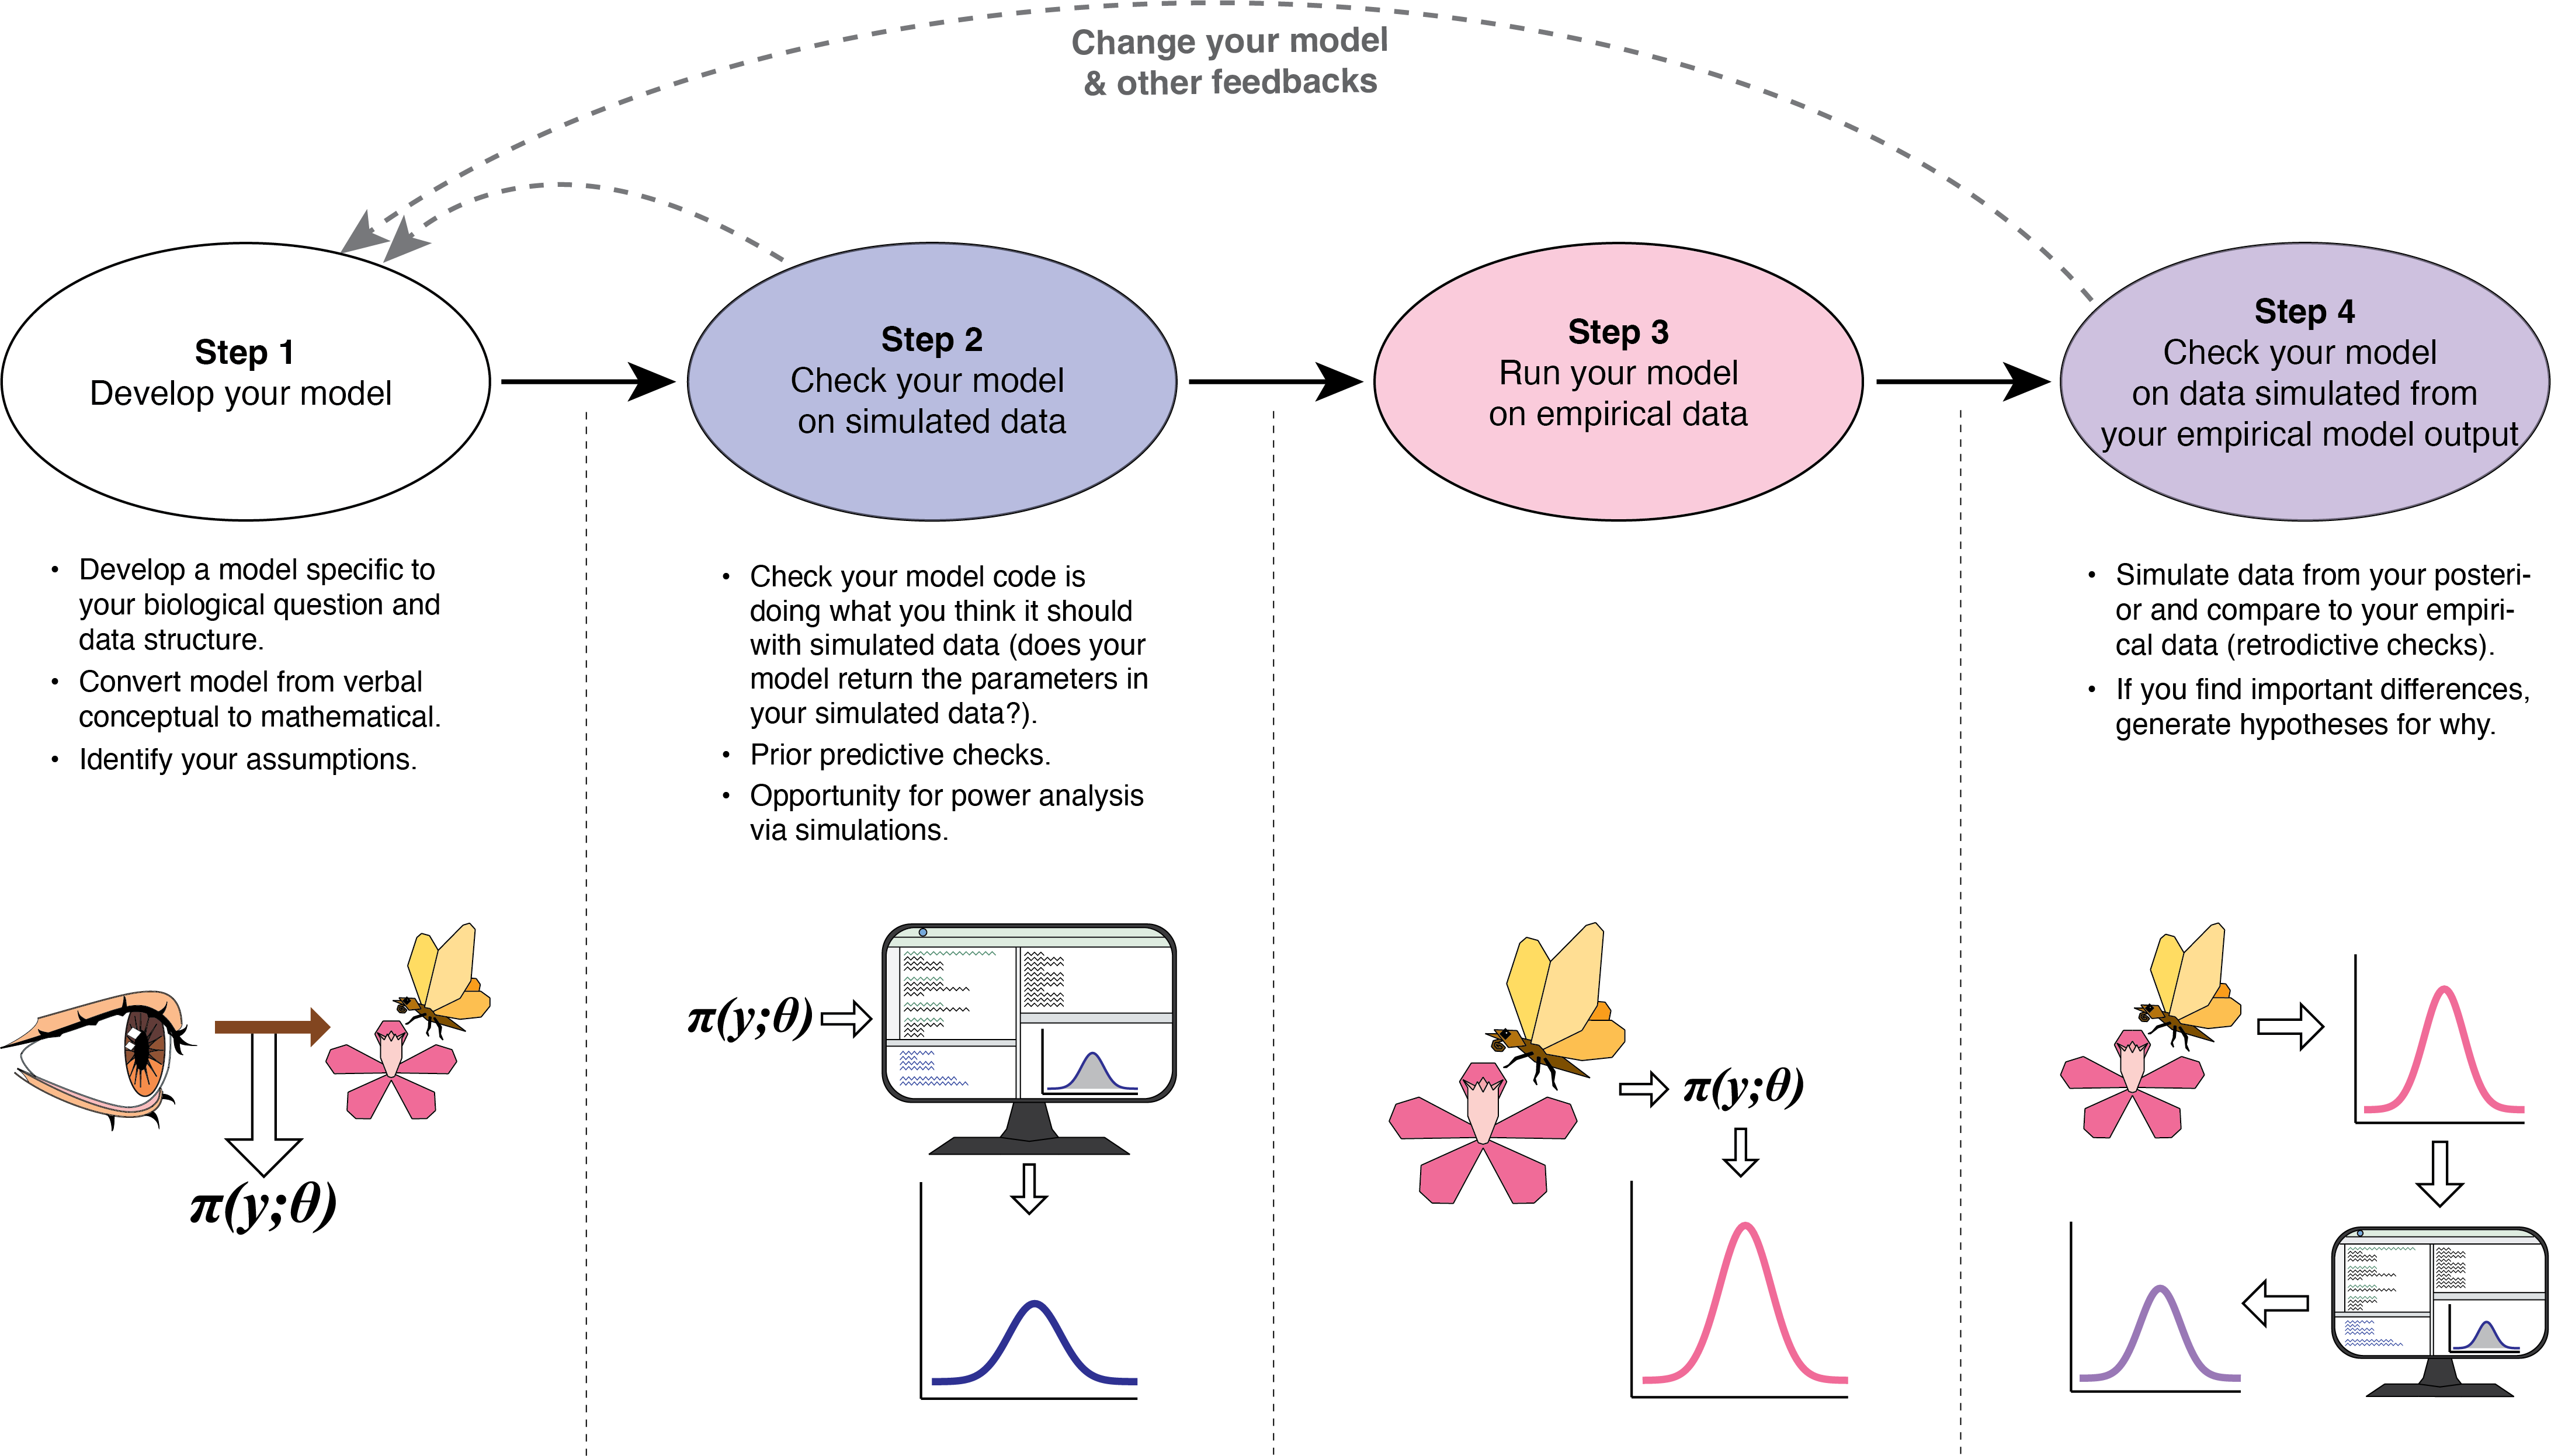
\includegraphics[width=1\textwidth]{figures/workflow.png}
\caption{The four-step iterative workflow we outline can help design models for specific ecological questions, data and aims---which makes this a statistical workflow that can naturally become a scientific workflow. It makes the step that many of us focus on---running your model on your empirical data (Step 3)---far more straightforward and insightful by using simulations both before (Step 2) and after (Step 4) it to better understand the model and data together.}
\label{fig:workflow}
\end{figure}

\begin{figure}[ht]
\centering
\noindent 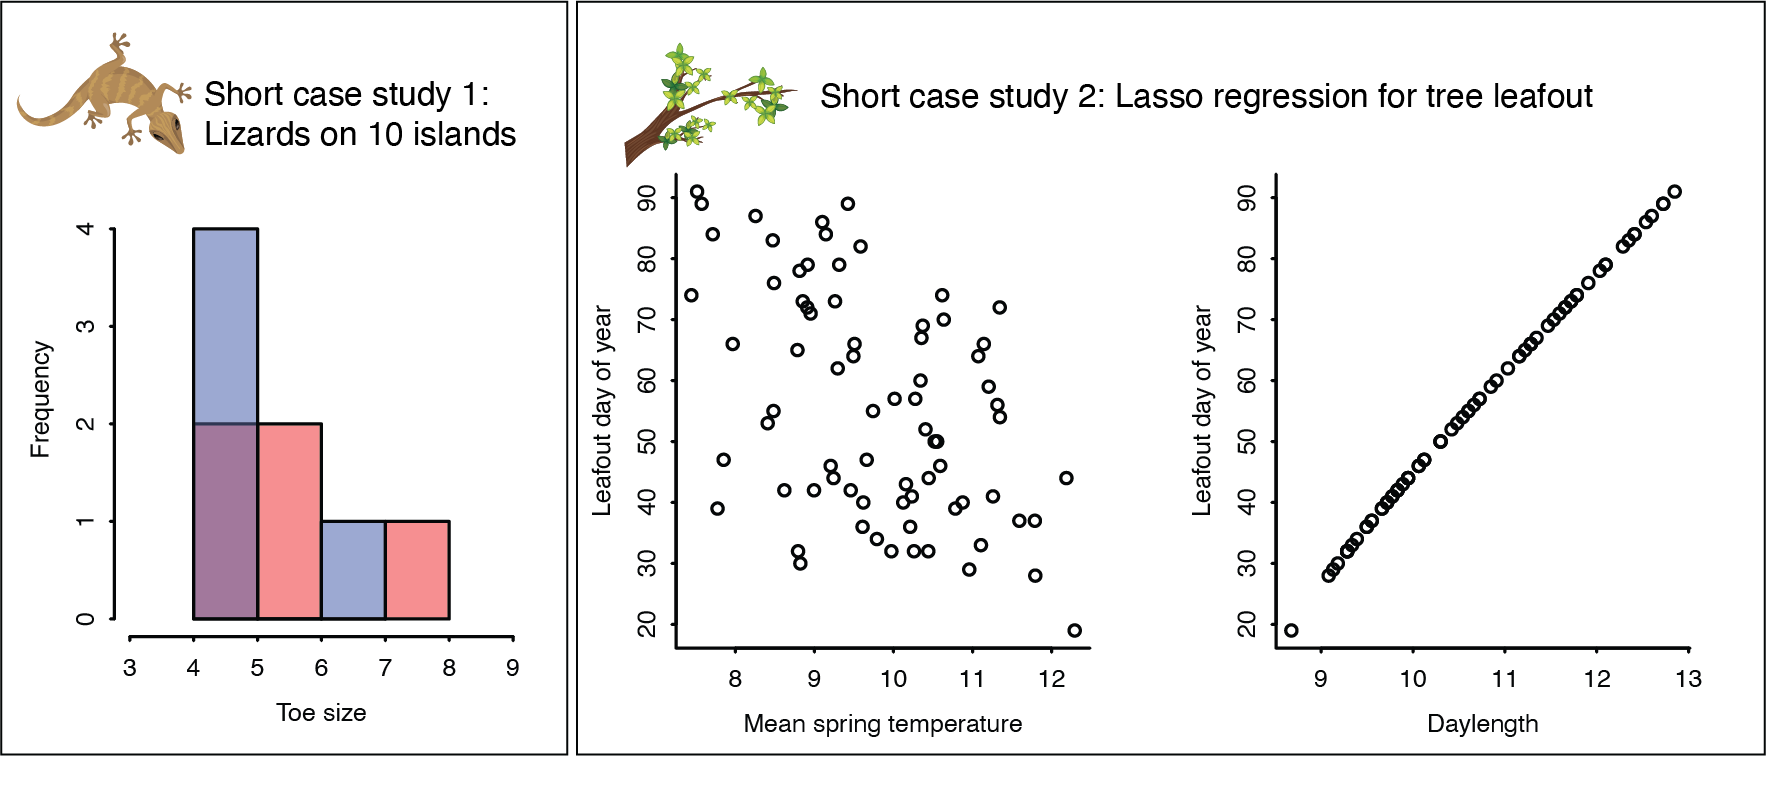
\includegraphics[width=0.7\textwidth]{figures/twoexamples.png}
\caption{We provide three very simple examples of the first steps of this workflow as Supplements (in PDF from R Markdown files). One example (a) uses ordinary least squares regression considering a natural experiment on lizards on tropical islands, and simulating two different possible sample sizes. The next example (b) uses lasso regression to examine how environmental variables may predict tree leafout. The third example (c) shows several examples of non-identifiability in regression models. See links within the Supplement: `Is a sample size of five stormy islands enough?'; `Identifying predictors of tree leafout' and `Three non-identifiable models, two of which are vital in biology.'}
\label{fig:twoexamples}
\end{figure}

\begin{figure}[ht]
\centering
\noindent 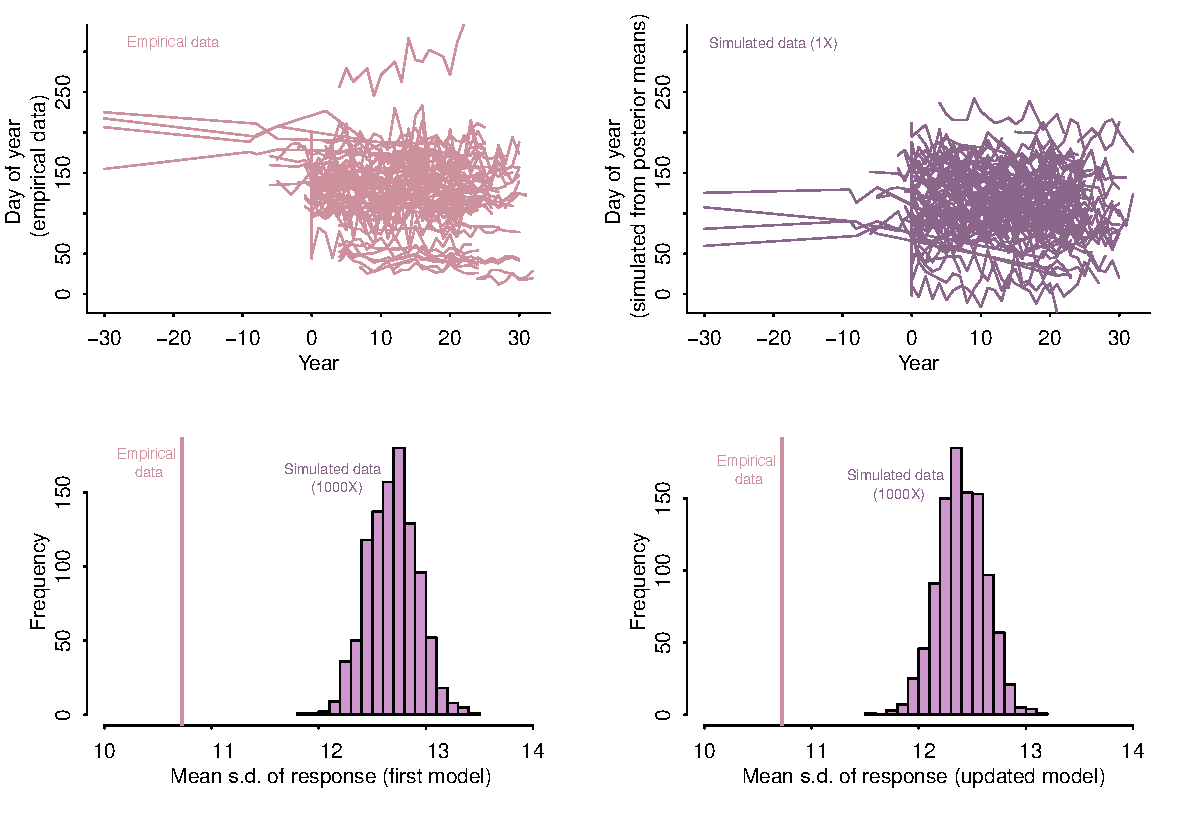
\includegraphics[width=0.95\textwidth]{examples/synchrony/graphs/fourpanelforpaper.pdf} 
\caption{Example of retrodictive checks (Step 4) and feedbacks from time-series data of phenological events over time. The empirical data (top left, pink) looks similar to one simulated dataset (top right, purple), based on existing species number, their respective $x$ data, and simulating from the parameters for each species, but the spread of the simulated data seems possibly higher. Repeating this retrodictive (or posterior predictive) check 1000 times, and taking the standard deviation (SD) of each simulated dataset, then looking at the resulting histogram confirms this (lower left in purple, empirical data SD in pink). This leads to an updated model, where the same retrodictive check looks slightly closer to the empirical data (lower right), but clearly still could be improved as part of additional feedbacks. These examples are shown in full in `Steps 1-4 in a Bayesian framework' linked in the Supplement.}
\label{fig:retrodictivecheck}
\end{figure}

\end{document}

